\documentclass[journal]{IEEEtran}
\usepackage{graphicx} % Required for inserting images
\usepackage{hyperref}
\usepackage{float}

\begin{document}

\begin{center}
   \Large Garden Automated Rain/Daylight Executed by Near-Infrared Sensing \break

   \large Nicholas Chitty, Brendan College, Scott Peirce, Justin Pham-Trinh \break

   \large University of Central Florida, Dept. of Electrical and Computer Engineering, Orlando,
   Florida, 32816-2450
\end{center}

\begin{abstract}
   This paper will show the application of near infrared spectroscopy 
and how it can measure electromagnetic waves from the emission of soil. Near infrared spectroscopy 
is an absorption spectroscopy method that can help determine the chemical composition of a 
substance through the radiation the substance gives off. Soil itself is a mixture of organic and 
inorganic substances that all together directly contribute to a garden’s environment. We are 
starting with soil with unknown qualities, so comparisons will be made between our soil and soil 
of known qualities to match and ensure that our plant is in a healthy and suitable environment. 
\end{abstract}

\section{Introduction}
\IEEEPARstart{I}{n} the past year, we have seen a great increase in remote sensing, wireless 
communication, API integration, and so much more. All of which have been made more available and 
economical. The internet has also seen its share of ``DIY" projects and its continuing growth.

In the agriculture industry, there have been new advancements in technology with high performance 
water distribution, network communication, and remote sensing. This research is intended to advance
the field by producing a system that can maintain a suitable environment for a plant to grow. In the 
environment, there will be sensors that will help modify the conditions within the environment. In 
addition to this system, it will feature a web interface for notifications and the ability for the 
user to set settings.

Monitoring soil isn't always the most fun or the easiest task, because things could get dirty or we 
might forget about our plant. This project will feature an on-the-rise technology in the form of a 
spectrophotometer. Smart systems nowadays are big learning machines that are constantly aware of its 
surroundings. For a smart agricultural system, it would need to determine variables such as moisture 
levels, nutrient content, pH levels, and so much more. This paper will introduce near infrared 
spectroscopy as another method to soil sensing that may prove to be more beneficial over traditional 
products or techniques.

This project will also present other fields such as system controls, power, and web, all to provide 
a "set it and forget it" home gardening experience. A home gardening experience where the garden bed 
can communicate with the user and the user can provide instruction of what to do, but also at the 
core, this is a microcontroller project that anybody can do with just slight knowledge and understanding
of digital communications. Like any smart device too, the internet plays an important role in making 
this as hands-off as it can be. There are many different communication protocols such as Bluetooth, 
Zigbee, Thread, and even short-range/long-range protocol. For this project we decided to go with WiFi 
because of its decreased bandwidth and that we aren't expecting to produce or receive large amounts 
of data. 

An important aspect to a lot of devices as well is data storage and web usage. This is important so 
that we can look back on previous information and make observations and conclusions. With our 
microcontroller, the web system is going to communicate with it through transmission control protocol.
Transmission control protocol is a standard on how to establish and maintain a network connection to 
exchange data. The web system will also have 16gb database to store data and have the ability to support 
multiple garden beds in a scaled solution. As mentioned before, the web system will have a feature to 
allow the user to set settings but also read the data that is stored. Lastly, an important factor to 
any garden is the weather and knowing when it might be cold, hot, or even rain outside. As a part of 
our web system, it will communicate using HTTP requests with a weather service to receive updates on 
the weather.

Solar power has been a growing source of energy for the past years and still continues to be with new 
developments and breakthroughs with solar technology. A lot of systems nowadays are solar powered but 
these products are not constantly in use, they have to turn of eventually. When the product is off the 
solar panel can still collect energy which is stored in a battery for conservation. In this paper, we 
will demonstrate our system running independently, battery powered but charged through solar panels.

In all, this paper will present how near infrared spectroscopy can be used to monitor a plant's environment 
and notify users with information of its health. Generating and guiding electromagnetic waves into a 
housing, scanning the substance, and then converting this optical power into a voltage that can be 
read and analyzed. It is then the microcontroller will communicate with the web system, storing the 
information and deciding on if anything needs to be done and notifying the user. 
\subsection{Goals} \label{sec:goals}
The following are the goals the team set for themselves with this project. Starting with non-
negotiable goals:
\begin{enumerate}
   \item A spectrometer that operates in the 400nm to 1700nm band with a spectral resolution less
         than 50nm and signal-to-noise ratio greater than 2.
   \item The ability to automatically feed water into the garden bed.
   \item Serve data to the user.
\end{enumerate}
Moving on, the team had goals they hoped to accomplish:
\begin{enumerate}
   \item Power the garden bed completely from solar and battery power.
   \item Serve data to the user via a website.
\end{enumerate}
\section{High-Level Design}
Based on the goals listed in \autoref{sec:goals} this section will discuss the high-level thought
process the team undertook in achieving those goals.
\begin{figure}[H]
    \centering
    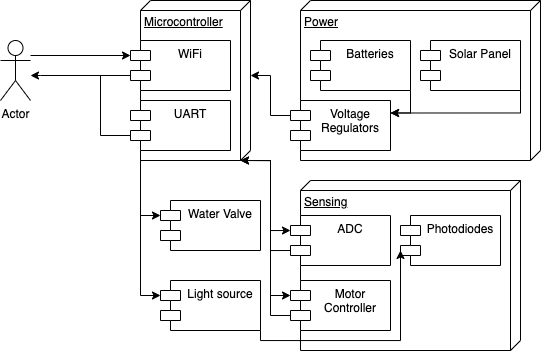
\includegraphics[width=\linewidth]{images/Flowchart.png}
    \label{fig:flowchart}
    \caption{The large systems and their interfaces and submodules}
\end{figure}
Figure \ref{fig:flowchart} the actor is any user. The team labelled both UART and WiFi blocks as interfaces to the user
because as of the time of writing, the web server is not serving live data. In the figure, sensing is used interchangeably with spectrometer.
\subsection{Spectrometer} 
In most instances, spectrometers are designed using charged couple devices in an array which some
component such as a prism or diffraction grating will shine upon breaking the source into its
components. This approach would be prohibitively expensive for such a consumer-oriented garden
bed. The solution was to use either a photodiode or photoresistor to measure the magnitude of the
of optical power in a given area\cite{Cao}. This sensor could be moved in order to give the effect of shining
the source on an array with the only major downside being the duration needed to scan. Find below a 
generalized block diagram for how this subsystem works.
\begin{figure}[H]
    \centering
    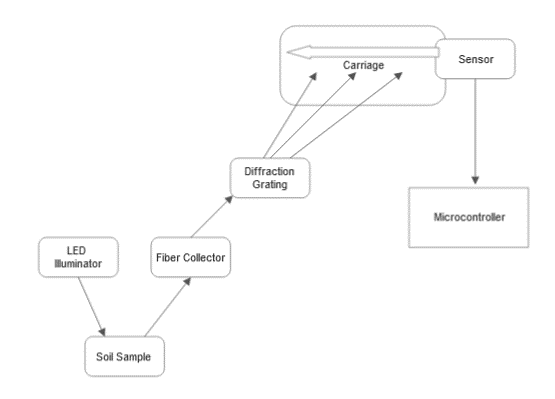
\includegraphics[width=\linewidth]{images/OpticsBlockDiagram.png}
    \label{fig:sensing-block}
    \caption{Diagram showing the major components of the sensing subsystem.}
\end{figure}
\section{Major Components} \label{sec:major-components}
The components found in this section make up the logical boundaries between systems and their
subsystems.
\subsection{Photosensitive device}
The first major decision regarding components comes down to the choice between using a photodiode versus
a photoresistor. The main advantage to photodiodes is their increased sensitivity. These means that with a lower
optical power on the photosensitive surface, the electrical output should be higher by comparison to the photoresistor.
This is a large consideration when understanding that soil will have a very low albedo (fraction of light a surface reflects)
which means that every photon that hits the detector needs to have an effect.
Thus the team chose two different photodiodes, the BPX 61 for the visual spectrum, and an InGaAs photodiode from Thor labs
for near-infrared light.
\subsection{Light source}
The selection of the light source is important in that the light source needs to emit the wavelengths
of light to be measured in roughly equal quantities. Based on the team's research tungsten lamps are a good source
of broad spectrum light especially at optical power levels with respect to the necessary electrical input.
\subsection{Linear Rail}
Referring to our high-level design, the team needed a linear rail with a sled that the sensors could be mounted to.
The team found such a device on Amazon.
\subsection{Water valve}
As part of the goals, the team wanted to be able to control the flow of water
into the plant bed. To accomplish this, they chose a solenoid valve whose rated pressure was well specificied for use with home water pressures.
\section{Hardware Detail}
In \autoref{sec:major-components}, a high level overview of components and features were given. This
section will discuss the implementation details of the chosen components.
\subsection{Spectrometer}
The spectrometer is comprised of 5 major components, the photosensitive device, the linear rail and motor controller, the analog-to-digital converter, and the light source. The light source is connected via a Darlington transistor as it is driven with a 12V supply @ 1.7A. The darlington transistor will keep separate this electrical supply from the digital logic to control the lamp. The light source is fed into a fiber optic cable and pointed at a patch of soil which will reflect light into a secondary fiber optic cable.
This project involves a large diffuse source, the illumined soil. The Fiber collimator will be attached to the fiber cable via their SMA connectors, then the collimator will be set in an acrylic block so that it rests 8.06mm above the soil. The block will also have a slot for the Light source to illuminate the soil at an angle, similar to the arrangement of the source and sensor in a computer mouse above a mousepad.
The signal will travel through the fiber and up into the spectrometer housing, where the other connector of the cable will be mounted in place. Another collimator will take the output beam and collimate it so that it propagates through free space into the housing. The collimator has an output beam diameter of 1.7mm. This planar wavefront will strike the diffraction grating.
We will call to the first optic cable as the source, and the second cable as the signal. From the signal cable, the light is transmitted onto a diffraction grating. This diffraction grating will split all the wavelengths of light across a rotational area of 47\textdegree. At this point, the team can do simple trigonometry to translate a linear position to a range of wavelengths being scanned. The team chose for the sensor to be at a distance of 30mm from the diffraction grating. 
\begin{figure}[H]
    \centering
    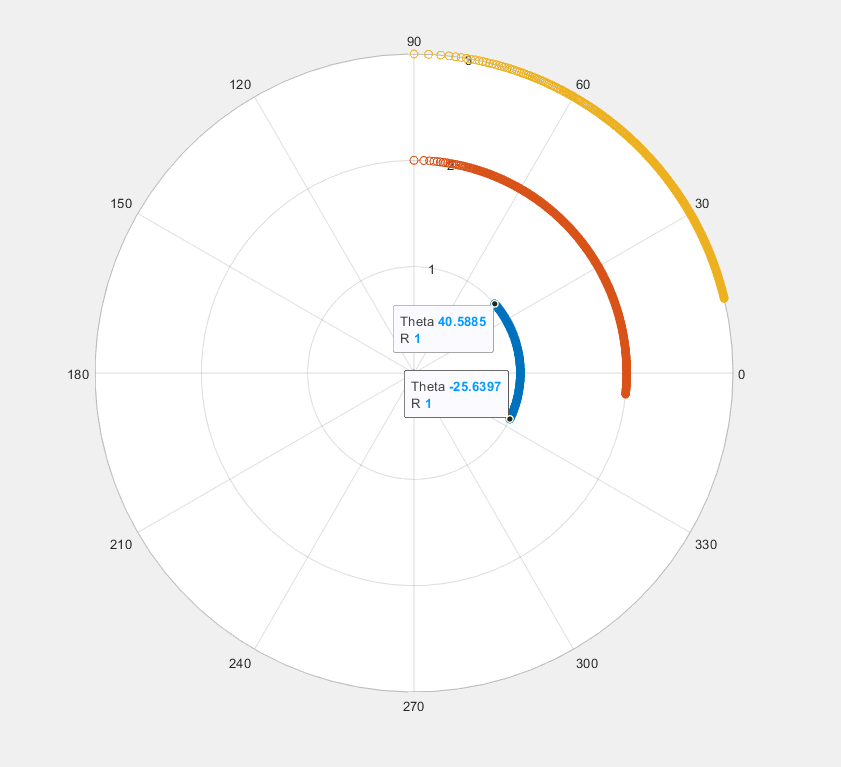
\includegraphics[width=\linewidth]{images/DiffractionAngleCalculator.png}
    \label{fig:diffraction-angle}
    \caption{The diffraction angle of 1st through 3rd order diffractions.}
\end{figure}

It is at this point that the spectrometer design enters the electrical domain. Due to the
photosensitive device being a photodiode where the current is a result of the optical power on the
sensitive area, the team built a current-to-voltage converter which would be fed into the
analog-to-digital converter. The primary issue at this point is just how small the optical power of
the light is. Given that the sensors have a translation of 1nA/1mW of power, we needed to design a
high gain, low noise converter. We chose 100e6 for the gain meaning that 1nA would translate to
100mV which is over double the resolution of our 16-bit ADC.
\begin{figure}[H]
    \centering
    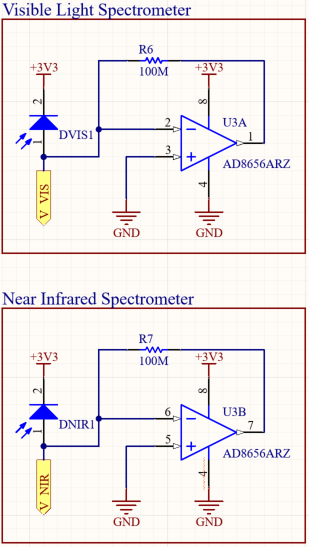
\includegraphics[height=.25\textheight]{images/SensorSchematics.PNG}
    \label{fig:sensor-schematic}
    \caption{The schematics for the current-to-voltage converter.}
\end{figure}
The net labelled \verb|V_NIR| and \verb|V_VIS| are sandwiched between ground planes on their track
to the ADC to reduce noise caused by electrostatic discharge or other analog signals (such as the
motor current). Before being read by the ADC the team designed a low pass filter to try to attenuate
the noise above 60Hz. The value of 60Hz was chosen as the cut off frequency because during
testing the oscilloscope showed a signal frequency in that range that would be detrimental to the
readings.
\section{Software Detail}
The microntroller serves as the glue holding this design together. In this section the means of
integrating the various subsystems via software will be discussed.
\subsection{Motor Controller}
To drive a DC motor we similarly needed a device to separate the digital logic from the back emf of the motor. This is done through the use of the motor driver. The timing of the signals is the most important part as the driver is just using the current and voltage source designed specifically for the motor in the timings given by the input pins. Wrong timing leads to the ability to skip tests leading to indeterministic behavior. The issue is the the CC32xx SDK abstracts away a lot of the fine tunability of setting hardware registers. To resolve this, the team used the specific board's hardware driver implementation to set the output on the pins with a delay of only 28 cycles. COMBINE WITH BRENDAN'S SECTION ON THE TOPIC
\bibliographystyle{ieeetr}
\bibliography{references/sensing}
\end{document}